\chapter{Measurements}\label{ch:results}

To test the system a few measurements had to be done. The measurements relate especially to GNSS, because the GNSS module by Cohda Wireless was not accurate enough. 

\section{Localization}

On big parking areas, the supplied GNSS module can determine a single parking lot as seen in figure \ref{fig:ppfitcohda}. The orange rectangle represents a parking lot of 2.25\;m width and 5.5\;m length.

\begin{figure}[htb]
	\centering
	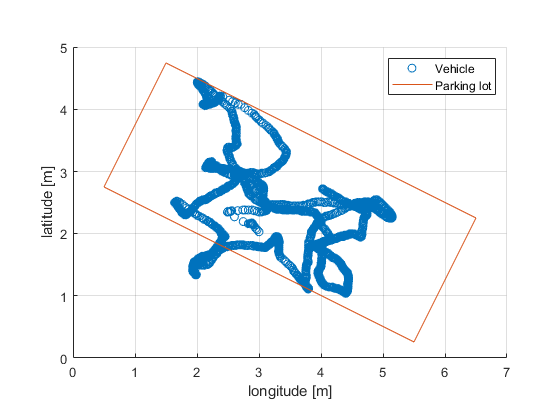
\includegraphics[width=0.85\textwidth]{images/ppfitcohda}
	\caption{Accuracy of the Cohda Wireless GNSS system. }
	\label{fig:ppfitcohda}
\end{figure}

\newpage

But on the HSR campus, where the charging device is mounted, the positioning system gets worse. The localization within a single parking lot is impossible in certain places. There are two GNSS repeaters installed at HSR. Both were suspected as possible sources of interference. The repeater sends signals received at its location. Therefore, they differ from the signal received by the GNSS module directly from the satellites. Turning off the repeaters did not entail the desired improvements. Both did not affect the localization, when the vehicle is parked next to the room. Multiple measurements were done to compare conditions with the repeaters switched on and off. The conditions at the parking lot next to the charging station are shown in figure \ref{fig:repeateronoff}.

\begin{figure}[htb]
	\centering
	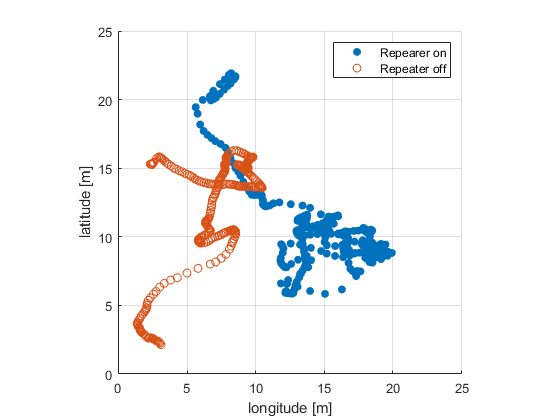
\includegraphics[width=0.7\textwidth]{images/repeateronoff}
	\caption{Comparison of the GNSS Accuracy with the Repeater switched on and off without RTK}
	\label{fig:repeateronoff}
\end{figure}

\begin{figure}[htb]
	\centering
	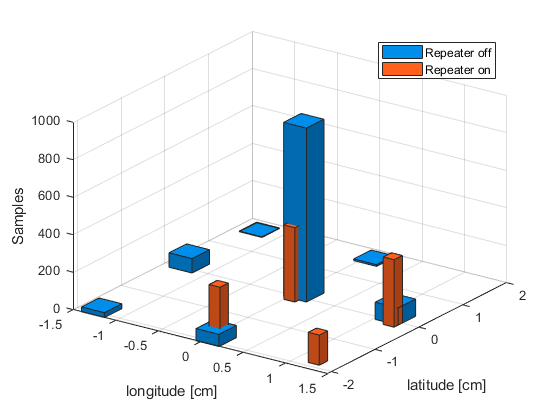
\includegraphics[width=0.6\textwidth]{images/2DHistRepOnOff}
	\caption{Comparison of the GNSS Accuracy with the Repeater switched on and off with RTK}
	\label{fig:RepOnOff}
\end{figure}

\newpage

Figure \ref{fig:RepOnOff} shows a 2-dimensional histogram to compare RTK measurements with the GNSS repeater switched on and off. Just as without RTK, the repeaters does not affect the accuracy neither in this case.

Another possible reason for the errors is reflection. The buildings in the HSR are situated close to each other and contain a lot of metal. The surface of the buildings reflect the GNSS signals, which leads to multipath conditions.

\newpage

An approach to fix this problem was to measure the location of the RSU and the OBU and use only the difference of both devices. Similar to a differential GNSS. If both positioning systems have the same drift, the errors can be calculated. Then the vehicle position can be determined by calculating the distance between both units. But this does not work with the Cohda Wireless GNSS modules, as seen in figure \ref{fig:diffmessung}. It shows the measured Euclidean distance of the OBU and RSU if both devices are stationary placed next to each other. The real measured distance was 2\;m. Its value changed too much to get any useful data. Therefore, this approach did not bear a solution.

\begin{figure}[htb]
	\centering
	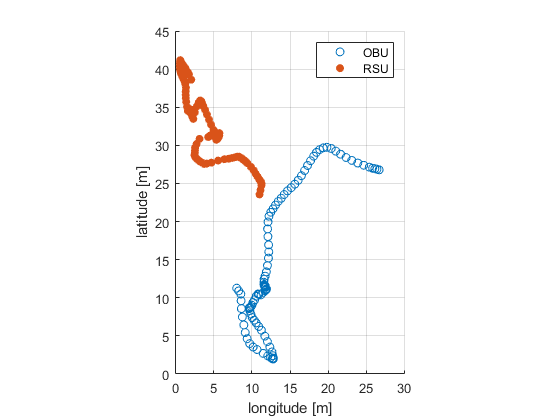
\includegraphics[width=0.65\textwidth]{images/OBURSUDrift}
	\caption{GNSS Drift during the Test}
	\label{fig:OBURSUDrift}
\end{figure}

\begin{figure}[htb]
	\centering
	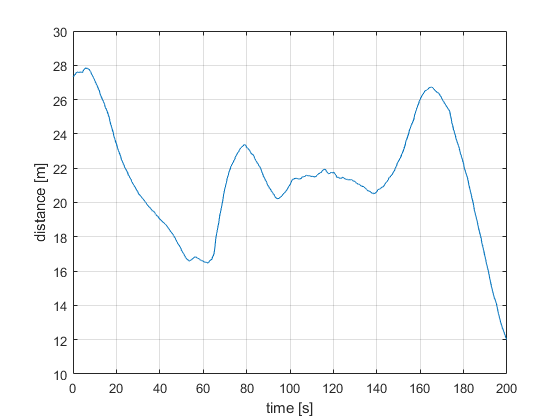
\includegraphics[width=0.6\textwidth]{images/diffmessung_pp}
	\caption{Measured Distance between OBU and RSU}
	\label{fig:diffmessung}
\end{figure}

Both units drift in different directions as seen in figure \ref{fig:OBURSUDrift}. Therefore the RSU can not detect the GNSS drift to calculate the exact vehicle position. Both figures above shows log data from the same measurement.

\clearpage
\pagebreak

\section{Real Time Kinematic}

The GNSS module by Cohda Wireless is not able to solve this problem. Therefore another module has to be implemented. To get really accurate positioning an RTK module is chosen.

Four situations were measured to find out whether RTK or the repeaters have an impact on accuracy. This measurement was done with a ZED F9P u-blox module. 

\begin{figure}[htb]
	\centering
	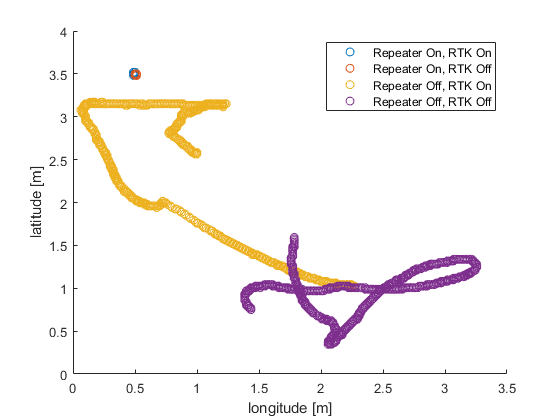
\includegraphics[width=0.9\textwidth]{images/GPSDriftComparison}
	\caption{Localization Measurement on the HSR Campus}
	\label{fig:4comp}
\end{figure}

Figure \ref{fig:4comp} shows, that the repeater has no significant impact proper localization. But both RTK measurements are very accurate. This test was done on a forecourt next to a tall building. Without RTK, similar drift movements occur compared with the GNSS module by Cohda Wireless.

\clearpage
\pagebreak

\begin{figure}[htb]
	\centering
	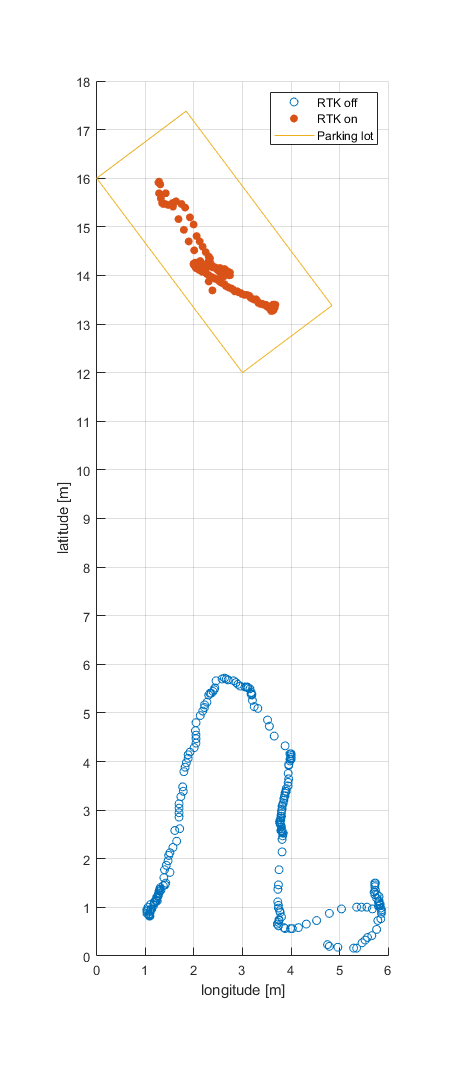
\includegraphics[width=0.5\textwidth]{images/ppfitRTKOnOff}
	\caption{Measurement at the Parking Lot next to the Charing Device}
	\label{fig:ppfitRTK}
\end{figure}

The measurement in figure \ref{fig:ppfitRTK} was done with the vehicle on the parking lot next to the charging device. The vehicle stands at the same position for both measurements. The one with RTK has less drift and is more accurate. It is less accurate than on open squares but to detect a single lot it is enough.

\clearpage
\pagebreak

\begin{figure}[htb]
	\centering
	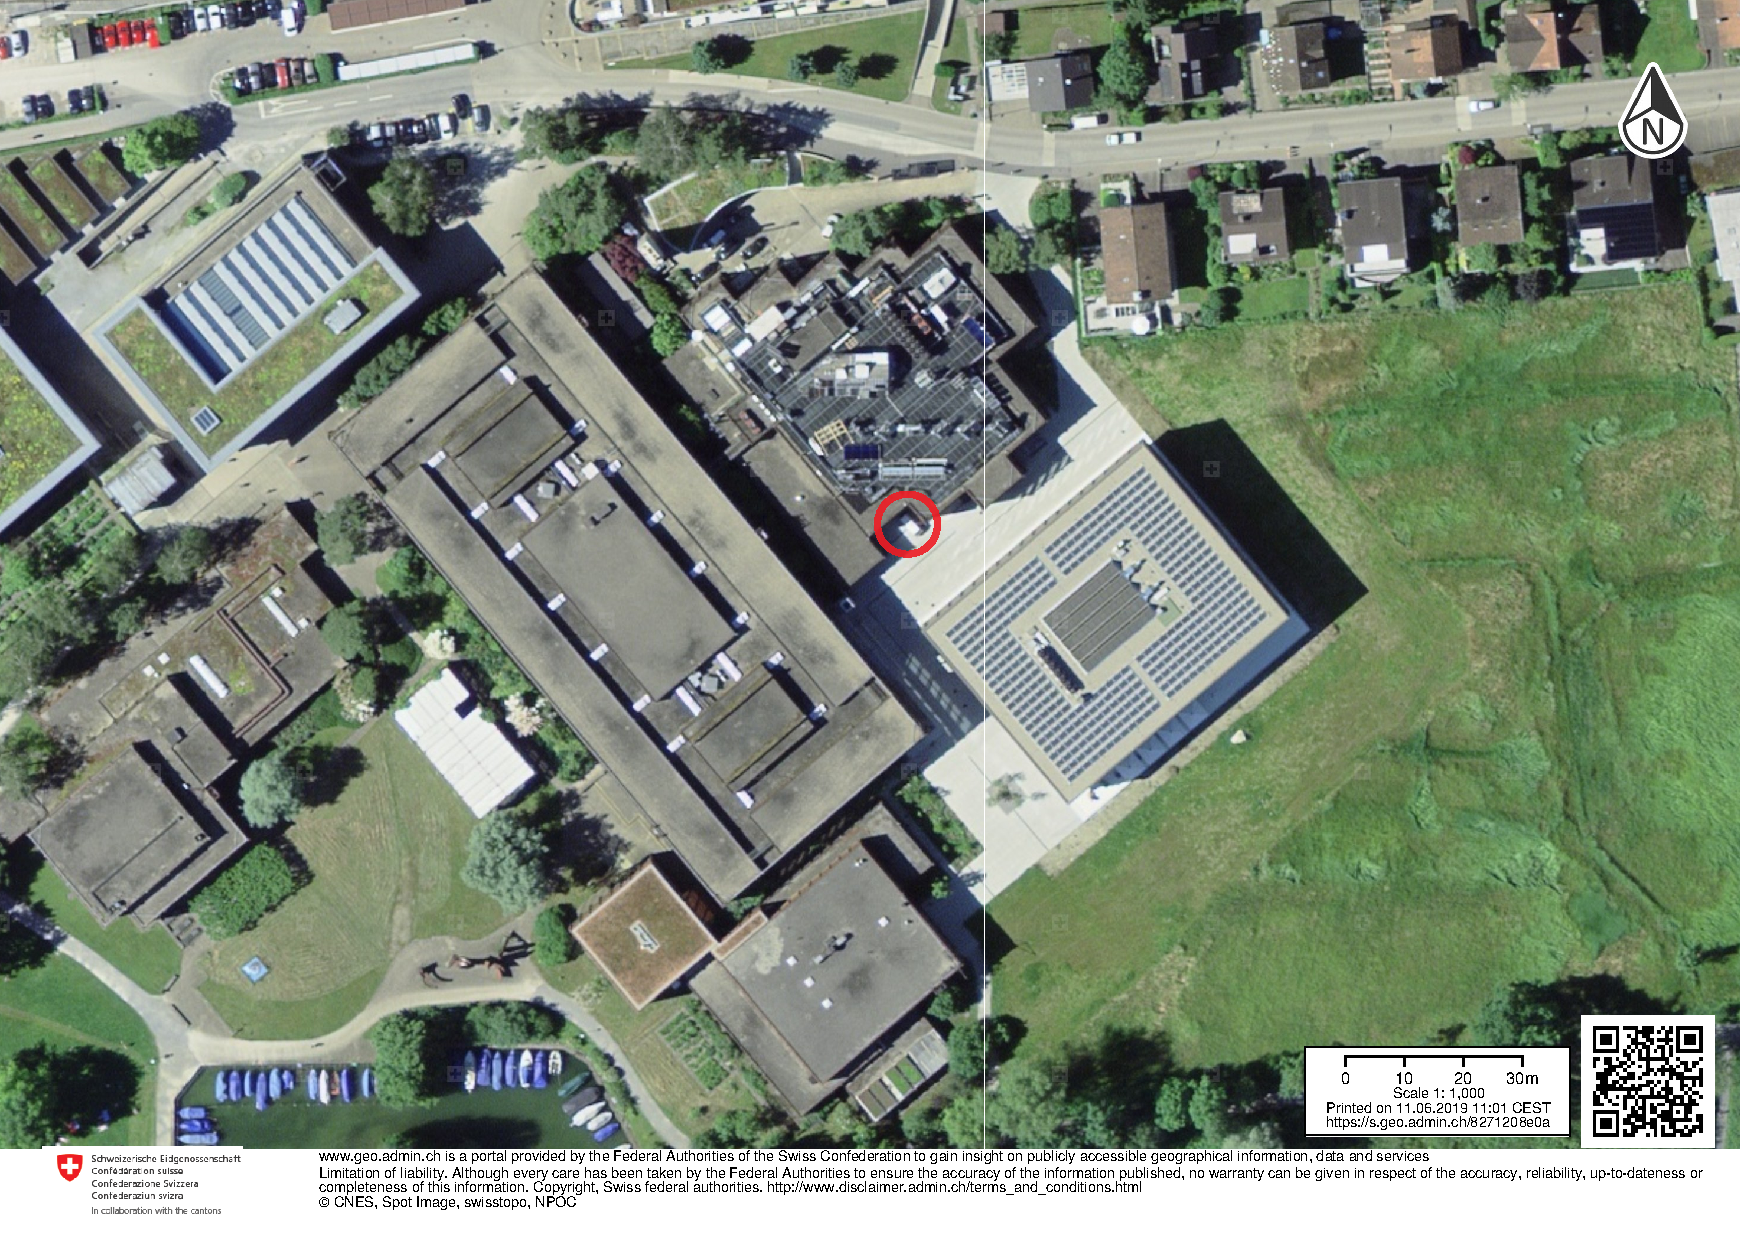
\includegraphics[width=0.9\textwidth]{images/mapHSR}
	\caption{Parking Lot next to the Charging Device}
	\label{fig:mapHSR}
\end{figure}

The red circle in figure \ref{fig:mapHSR} shows the difficult location where the vehicle is parked. The parking lot is between multiple tall buildings.

Despite these conditions, a single parking lot can be determined by the precision improvement with RTK.
The car can be located with an accuracy of 2\;cm. This is much more precise than needed for this application, but it was achieved without any additional effort. The estimated accuracy during a ride is shown in figure \ref{fig:rtkhf}.

The RTK base station has a minimum accuracy of 5\;cm. This error adds up to the 2\;cm precision of the vehicle. The outcome of this is an overall error equal to 7\;cm in the worst case. For future projects with RTK, this base station can be used a few kilometers around the university.

With a cold start of the rover it takes about 25\;s to get a 3-dimensional fix. After the correction data was received, it takes several minutes to get a differential fix. This is not necessary because a differential float condition is accurate enough for this project. Figure \ref{fig:AccSt} shows how the accuracy improves after a start. \cite{RTK_FIX/FLOAT}

\subsection*{Conclusion}

The implementation of an RTK system was the solution. With correction data of the RTK base station, the error could also be minimized for tough environments. With RTK it was possible to locate a vehicle precise enough to determine on which parking lot it is parked.

\section{Range Test of the V2X Channel}
The range of the Cohda Wireless V2X channel was tested over an open field and through buildings. A ride around the campus was driven, to check where both units can communicate with each other. The transmit power of 23\;dBm (200\;mW) was used for this test. The charging station was placed on a square next to a field to give proper circumstances for a range test.
\cite{CohdaWirelessETSA}

\begin{figure}[htb]
	\centering
	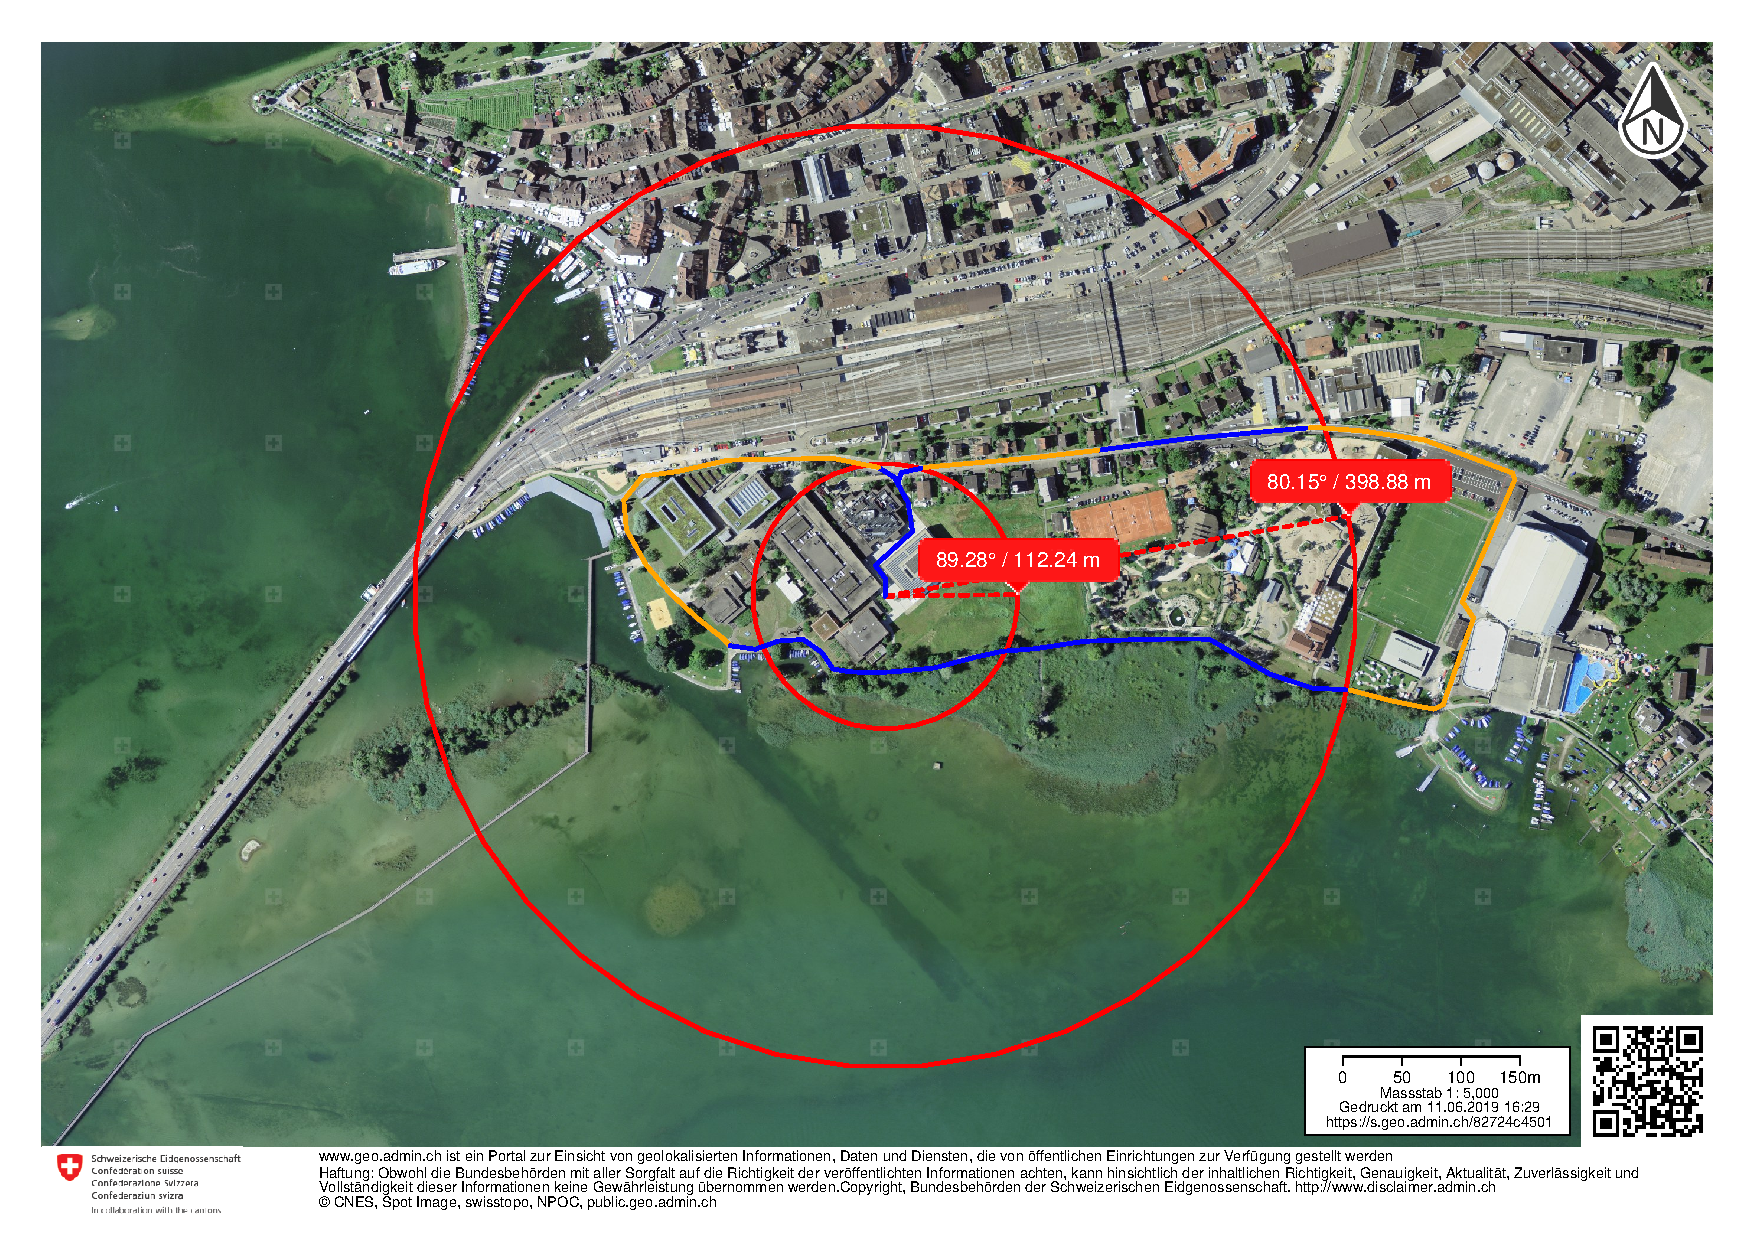
\includegraphics[width=1\textwidth]{images/rangetest}
	\caption{V2X Channel Range Test}
	\label{fig:rangetest}
\end{figure}

The inner circle represents the range without line of sight and the outer one the range with line of sight. On the blue track, the communication is possible and stable, on the orange one it is not possible.
